\documentclass[10pt,twocolumn,letterpaper]{article}

\usepackage{iccv}

% This is roughly version 1.1 of vcl-shortcuts, circa Dec 2016.
% Put together by Vladlen Koltun

\usepackage{times}
\usepackage{epsfig}
\usepackage{graphicx}
\usepackage{float}
\usepackage{wrapfig}
\usepackage{amsmath,amssymb,amsthm}
\usepackage{algorithm,algorithmicx,algpseudocode}
\usepackage{bm,xspace}
\usepackage{comment}
\usepackage{verbatim}
\usepackage{multirow}
\usepackage{balance}
\usepackage{url}
\usepackage{booktabs}
\usepackage{etoolbox,siunitx}
\usepackage{calc}
\usepackage{pifont,hologo}
\usepackage[usenames, dvipsnames]{color}
\usepackage{nicefrac}

%Set up nice tables using the tabular package
%Make \toprule and \bottomrule thicker than \midrule
\setlength\heavyrulewidth{0.10em}
\setlength\lightrulewidth{0.05em}
\setlength\cmidrulewidth{0.03em}
\newcommand{\ra}[1]{\renewcommand{\arraystretch}{#1}}

%Set up the siunitx package, particularly for using the S column type in tables
\usepackage[super]{nth}
\usepackage{nicefrac}
\sisetup{detect-weight=true,detect-inline-weight=math}
\sisetup{quotient-mode = fraction}
\sisetup{fraction-function = \nicefrac}
\robustify\bfseries

% AMS stuff
\usepackage{dsfont}


\newtheorem{theorem}{Theorem}
\newtheorem{lemma}{Lemma}
\newtheorem{cor}{Corollary}
\newtheorem{proposition}{Proposition}
\newtheorem{definition}{Definition}

\newcommand*{\eg}{e.g.\@\xspace}
\newcommand*{\ie}{i.e.\@\xspace}


%Known issue: the following shortcuts override \gg, \ll\, and \tt, which are existing LaTeX commands. Use \ggreater and \llesser, defined below, instead of \gg and \ll. Use \texttt{} instead of \tt.
%Also \ss is taken and in some environments cannot be overridden. Use \sss for a bold `s' instead.
\def\aa{\mathbf{a}}
\def\bb{\mathbf{b}}
\def\cc{\mathbf{c}}
\def\dd{\mathbf{d}}
\def\ee{\mathbf{e}}
\def\ff{\mathbf{f}}
\def\gg{\mathbf{g}}
\def\hh{\mathbf{h}}
\def\ii{\mathbf{i}}
\def\jj{\mathbf{j}}
\def\kk{\mathbf{k}}
\def\ll{\mathbf{l}}
\def\mm{\mathbf{m}}
\def\nn{\mathbf{n}}
\def\oo{\mathbf{o}}
\def\pp{\mathbf{p}}
\def\qq{\mathbf{q}}
\def\rr{\mathbf{r}}
\def\sss{\mathbf{s}}
\def\tt{\mathbf{t}}
\def\uu{\mathbf{u}}
\def\vv{\mathbf{v}}
\def\ww{\mathbf{w}}
\def\xx{\mathbf{x}}
\def\yy{\mathbf{y}}
\def\zz{\mathbf{z}}

\def\AA{\mathbf{A}}
\def\BB{\mathbf{B}}
\def\CC{\mathbf{C}}
\def\DD{\mathbf{D}}
\def\EE{\mathbf{E}}
\def\FF{\mathbf{F}}
\def\GG{\mathbf{G}}
\def\HH{\mathbf{H}}
\def\II{\mathbf{I}}
\def\JJ{\mathbf{J}}
\def\KK{\mathbf{K}}
\def\LL{\mathbf{L}}
\def\MM{\mathbf{M}}
\def\NN{\mathbf{N}}
\def\OO{\mathbf{O}}
\def\PP{\mathbf{P}}
\def\QQ{\mathbf{Q}}
\def\RR{\mathbf{R}}
\def\SS{\mathbf{S}}
\def\TT{\mathbf{T}}
\def\UU{\mathbf{U}}
\def\VV{\mathbf{V}}
\def\WW{\mathbf{W}}
\def\XX{\mathbf{X}}
\def\YY{\mathbf{Y}}
\def\ZZ{\mathbf{Z}}

\def\aA{\mathcal{A}}
\def\bB{\mathcal{B}}
\def\cC{\mathcal{C}}
\def\dD{\mathcal{D}}
\def\eE{\mathcal{E}}
\def\fF{\mathcal{F}}
\def\gG{\mathcal{G}}
\def\hH{\mathcal{H}}
\def\iI{\mathcal{I}}
\def\jJ{\mathcal{J}}
\def\kK{\mathcal{K}}
\def\lL{\mathcal{L}}
\def\mM{\mathcal{M}}
\def\nN{\mathcal{N}}
\def\oO{\mathcal{O}}
\def\pP{\mathcal{P}}
\def\qQ{\mathcal{Q}}
\def\rR{\mathcal{R}}
\def\sS{\mathcal{S}}
\def\tT{\mathcal{T}}
\def\uU{\mathcal{U}}
\def\vV{\mathcal{V}}
\def\wW{\mathcal{W}}
\def\xX{\mathcal{X}}
\def\yY{\mathcal{Y}}
\def\zZ{\mathcal{Z}}

\def\Ae{\mathbb{A}}
\def\Be{\mathbb{B}}
\def\Ce{\mathbb{C}}
\def\Le{\mathbb{L}}
\def\Ne{\mathbb{N}}
\def\Pe{\mathbb{P}}
\def\Qe{\mathbb{Q}}
\def\Re{\mathbb{R}}
\def\Se{\mathbb{S}}
\def\Te{\mathbb{T}}
\def\Xe{\mathbb{X}}
\def\Ye{\mathbb{Y}}
\def\Ze{\mathbb{Z}}

\def\btheta{{\bm\theta}}
\def\bzeta{{\bm\zeta}}
\def\bmu{{\bm\mu}}
\def\bZero{\mathbf{0}}
\def\bOne{\mathbf{1}}

\DeclareMathOperator*{\argmax}{arg\,max}
\DeclareMathOperator*{\argmin}{arg\,min}
\DeclareMathOperator*{\minimize}{minimize}
\DeclareMathOperator*{\maximize}{minimize}

\DeclareMathOperator{\sign}{sign}
\DeclareMathOperator{\rank}{rank}
\DeclareMathOperator{\trace}{tr}
\DeclareMathOperator{\diag}{diag}
\DeclareMathOperator{\diam}{diam}

\def\eps{\varepsilon}
\def\vphi{\varphi}
\def\vsigma{\varsigma}

\def\trans{^{\top}}
\def\deg{^{\circ}}

\def\th{^{\textnormal{th}}}
\def\st{^{\textnormal{st}}}
\def\nd{^{\textnormal{nd}}}

%\ggreater and \llesser replace \gg and \ll, which have been overridden
\newcommand\ggreater{\mathbin{>\!\!\!>}}
\newcommand\llesser{\mathbin{<\!\!\!<}}

%Checkmark and cross symbols for tables
\newcommand{\YesV}{\ding{51}}%
\newcommand{\NoX}{\ding{55}}%

%Use @ instead of , in long numbers in math mode. For example, use $10@000$ rather than $10,000$.
\DeclareMathSymbol{@}{\mathord}{letters}{"3B}

\newcommand\paren[1]{\left(#1\right)}
\newcommand\abs[1]{\left\lvert#1\right\rvert}
\newcommand\norm[1]{\left\lVert#1\right\rVert}
\newcommand\tuple[1]{\left\langle#1\right\rangle}
\newcommand\inner[2]{\langle #1, #2 \rangle}

%Use \timess instead of \times in the main lines of equations, but not in superscripts or subscripts. Use the regular \times in superscripts or subscripts.
\newcommand\timess{\mathbin{\!\times\!}}

%Known issue: \nicebar is not nice in PNAS format, use \bar if submitting to PNAS.
\newcommand\nicebar[1]{\mkern 4mu\overline{\mkern-4mu#1}}

%Replace ``\yourname" and ``Name" with your name
\newcommand\ozan[1]{\textcolor{blue}{Ozan says: #1}}
\newcommand\vladlen[1]{\textcolor{red}{Vladlen says: #1}}
\newcommand\creadych[1]{\textcolor{green}{Change in CR: #1}}
\newcommand\creadyadd[1]{\textcolor{cyan}{Add in CR: #1}}

%Paragraph heading with customizable vertical spacing. Modify the length inside \vspace to expand or contract the vertical offset preceding a new paragraph heading.
\newcommand\mypara[1]{\vspace{1mm}\noindent\textbf{#1}}

%Orient text vertically. Useful for tables and figures.
\def\rot#1{\rotatebox{90}{#1}}

%I use the self-indulgent \LaTeX operator mostly to illustrate an issue and a useful trick. The issue is that LaTeX operators eat the space that follows them, so if they occur in the middle of a sentence they eliminate the space separating the following word. But you can't just insert a space will-nilly (e.g., \LaTeX\ or \LaTeX~) because if the operator is followed by a punctuation mark then there shouldn't be a space. One solution is to write \LaTeX{}, which does the right thing but is easy to forget. The alternative, demonstrated here, is to define an operator with a name that ends with the forward slash. This also does the right thing and looks sufficiently distinctive to be memorable.
\def\latex/{\LaTeX}
\def\bibtex/{\hologo{BibTeX}}

%Miscellaneous \latex/ tips:
% To create an invisible character, use the \phantom command or its relatives: http://tex.stackexchange.com/questions/4519/how-do-i-create-an-invisible-character


% Include other packages here, before hyperref.

% If you comment hyperref and then uncomment it, you should delete
% egpaper.aux before re-running latex.  (Or just hit 'q' on the first latex
% run, let it finish, and you should be clear).
\usepackage[pagebackref=true,breaklinks=true,letterpaper=true,colorlinks,bookmarks=false]{hyperref}

\iccvfinalcopy % *** Uncomment this line for the final submission

\def\iccvPaperID{253} % *** Enter the ICCV Paper ID here
\def\httilde{\mbox{\tt\raisebox{-.5ex}{\symbol{126}}}}

% Pages are numbered in submission mode, and unnumbered in camera-ready
\ificcvfinal\pagestyle{empty}\fi
\begin{document}

%%%%%%%%% TITLE
\title{Photographic Image Synthesis with Cascaded Refinement Networks}

\setcounter{footnote}{1}

\author{Qifeng Chen\thanks{Intel Labs}~~\thanks{Stanford University}
%\\
%\textsuperscript{1}Stanford University
% For a paper whose authors are all at the same institution,
% omit the following lines up until the closing ``}''.
% Additional authors and addresses can be added with ``\and'',
% just like the second author.
% To save space, use either the email address or home page, not both
\and
Vladlen Koltun\footnotemark[2]
%\\
%\textsuperscript{2}Intel Labs
}

\makeatletter
\g@addto@macro\@maketitle{
  \begin{figure}[H]
  \setlength{\linewidth}{\textwidth}
  \setlength{\hsize}{\textwidth}
  \vspace{-7mm}
  \centering
 	\begin{tabular}{@{}c@{\hspace{1mm}}c@{}}
  \includegraphics[width=0.493\textwidth]{figures/Label_000027.png} &
  \includegraphics[width=0.493\textwidth]{figures/Ours_000027.jpg}\vspace{0mm}\\
  \includegraphics[width=0.493\textwidth]{figures/Label_000338.png} &
  \includegraphics[width=0.493\textwidth]{figures/Ours_000338.jpg}\\
\small (a) Input semantic layouts & \small (b) Synthesized images
 	\end{tabular}
  \vspace{1mm}
  \caption{Given a pixelwise semantic layout, the presented model synthesizes an image that conforms to this layout. (a) Semantic layouts from the Cityscapes dataset of urban scenes; semantic classes are coded by color. (b) Images synthesized by our model for these layouts. The layouts shown here and throughout the paper are from the validation set and depict scenes from new cities that were never seen during training. Best viewed on the screen.}
  \label{fig:teaser}
%  \vspace{2mm}
  \end{figure}
}
\makeatother

\maketitle
%\thispagestyle{empty}

%%%%%%%%% ABSTRACT
\begin{abstract}
We present an approach to synthesizing photographic images conditioned on semantic layouts. Given a semantic label map, our approach produces an image with photographic appearance that conforms to the input layout. The approach thus functions as a rendering engine that takes a two-dimensional semantic specification of the scene and produces a corresponding photographic image. Unlike recent and contemporaneous work, our approach does not rely on adversarial training. We show that photographic images can be synthesized from semantic layouts by a single feedforward network with appropriate structure, trained end-to-end with a direct regression objective. The presented approach scales seamlessly to high resolutions; we demonstrate this by synthesizing photographic images at 2-megapixel resolution, the full resolution of our training data. Extensive perceptual experiments on datasets of outdoor and indoor scenes demonstrate that images synthesized by the presented approach are considerably more realistic than alternative approaches.
\end{abstract}

%%%%%%%%% BODY TEXT

\section{Introduction}
\label{sec:introduction}
\section{Introduction}

Humans use different forms of communications such as speech, hand gestures and emotions. Being able to understand one's emotions and the encoded feelings is an important factor for an appropriate and correct understanding.


With the ongoing research in the field of robotics, especially in the field of humanoid robots, it becomes interesting to integrate these capabilities into machines allowing for a more diverse and natural way of communication. One example is the Software called EmotiChat~\cite{Anderson06areal-time}. This is a chat application with emotion recognition. The user is monitored and whenever an emotion is detected (smile, etc.), an emoticon is inserted into the chat window. Besides Human Computer Interaction other fields like surveillance or driver safety could also profit from it. Being able to detect the mood of the driver could help to detect the level of attention, so that automatic systems can adapt.\\
\let\thefootnote\relax\footnote{*F. Trier and P. Burkert contributed equally to this work.}


Many methods rely on extraction of the facial region. This can be realized through manual inference~\cite{4032815} or an automatic detection approach~\cite{Anderson06areal-time}.
Methods often involve the Facial Action Coding System (FACS) which describes the facial expression using Action Units (AU). An Action Unit is a facial action like "raising the Inner Brow". Multiple activations of AUs describe the facial expression~\cite{kumar2009face}. Being able to correctly detect AUs is a helpful step, since it allows making a statement about the activation level of the corresponding emotion. \\
Handcrafted facial landmarks can be used such as done by Kotsia et al.~\cite{4032815}. Detecting such landmarks can be hard, as the distance between them differs depending on the person~\cite{6998925}. Not only AUs can be used to detect emotions, but also texture. When a face shows an emotion the structure changes and different filters can be applied to detect this~\cite{6998925}.\\


\begin{figure}
   \centering
        \includegraphics[width=\columnwidth]{Fig1}
   \caption{Example images from the MMI (top) and CKP (bottom). The emotions from left to right are: \textit{Anger}, \textit{Sadness}, \textit{Disgust}, \textit{Happiness}, \textit{Fear}, \textit{Surprise}. The emotion \textit{Contempt} of the CKP set is not displayed.}\label{fig:example_images}
\end{figure}




The presented approach uses Artificial Neural Networks (ANN). ANNs differ, as they are trained on the data with less need for manual interference. 
Convolutional Neural Networks are a special kind of ANN and have been shown to work well as feature extractor when using images as input~\cite{donahue2013decaf} and are real-time capable. This allows for the usage of the raw input images without any pre- or postprocessing.\\
GoogleNet~\cite{DBLP:journals/corr/SzegedyLJSRAEVR14} is a deep neural network architecture that relies on CNNs. It has been introduced during the Image Net Large Scale Visual Recognition Challenge(ILSVRC) 2014. This challenge analyses the quality of different image classification approaches submitted by different groups. The images are separated into 1000 different classes organized by the WordNet hierarchy. In the challenge "object detection with additional training data" GoogleNet has achieved about 44\% precision~\cite{LSVRC-results}. These results have demonstrated the potential which lies in this kind of architecture. Therefore it has been used as inspiration for the proposed architecture.\\
The proposed network has been evaluated on the Extended Cohn-Kanade Dataset (Section~\ref{sec:ckp}) and on the MMI Dataset (Section~\ref{sec:mmi}). Typical pictures of persons showing emotions can be seen in Fig.~\ref{fig:example_images}.
The emotion \textit{Contempt} of the CKP set is not shown as no subject with consent for publication and an annotated emotion is part of the dataset. Results of experiments on these datasets demonstrate the success of using a deep layered neural network structure. With a 10-fold cross-validation a recognition accuracy of 99.6\% has been achieved. \\

The paper is arranged as follows: After this introduction, Related Work (Section~\ref{sec:related}) is presented which focuses on Emotion/Expression recognition and the various approaches scientists have taken. Next is Section~\ref{sec:background}, Background, which focuses on the main components of the architecture proposed in this article. Section~\ref{sec:datasets} contains a summary of the used Datasets. In Section~\ref{sec:architecture} the architecture is presented. This is followed by the experiments and its results (Section~\ref{sec:experiments}) . Finally, Section~\ref{sec:conclusion} summarizes the article and concludes the article.

\section{Related Work}
\label{sec:related}
\begin{comment}
      \begin{figure*}
      \centering
      \begin{tabular}{@{}c@{\hspace{1mm}}c@{}}
          \includegraphics[width=0.493\textwidth]{figures/Label_000167.jpg} &
          \includegraphics[width=0.493\textwidth]{figures/Label_000275.jpg}\vspace{0mm}\\
          \includegraphics[width=0.493\textwidth]{figures/Ours_000167.jpg} &
          \includegraphics[width=0.493\textwidth]{figures/Ours_000275.jpg}\vspace{0mm}\\
          \includegraphics[width=0.493\textwidth]{figures/Bekeley_000167.jpg} &
          \includegraphics[width=0.493\textwidth]{figures/Bekeley_000275.jpg}
      \end{tabular}
      \vspace{2mm}
      \caption{Comparison.}
      \label{fig:comparison}
      \vspace{2mm}
      \end{figure*}

      \begin{figure*}
      \centering
      \begin{tabular}{@{}c@{\hspace{1mm}}c@{\hspace{1mm}}c@{}}
          \includegraphics[width=0.330\textwidth]{figures/Label_000121.jpg} &
          \includegraphics[width=0.330\textwidth]{figures/Label_000343.jpg} &
          \includegraphics[width=0.330\textwidth]{figures/Label_000245.jpg}\vspace{0mm}\\
          \includegraphics[width=0.330\textwidth]{figures/Ours_000121.jpg} &
          \includegraphics[width=0.330\textwidth]{figures/Ours_000343.jpg} &
          \includegraphics[width=0.330\textwidth]{figures/Ours_000245.jpg}\vspace{0mm}\\
          \includegraphics[width=0.330\textwidth]{figures/Bekeley_000121.jpg} &
          \includegraphics[width=0.330\textwidth]{figures/Bekeley_000343.jpg} &
          \includegraphics[width=0.330\textwidth]{figures/Bekeley_000245.jpg}
      \end{tabular}
      \vspace{2mm}
      \caption{Comparison.}
      \label{fig:comparison}
      \vspace{2mm}
      \end{figure*}
\end{comment}

\begin{figure*}[t]
\centering
\begin{tabular}{@{}c@{\hspace{2mm}}c@{\hspace{2mm}}c@{}}
\rotatebox{90}{\hspace{11mm}Input layout}&
\includegraphics[width=0.46\linewidth]{figures/Label_000167.png} &
\includegraphics[width=0.46\linewidth]{figures/Label_000437.png}\\
\rotatebox{90}{\hspace{12.5mm}Our result}&
\includegraphics[width=0.46\linewidth]{figures/Ours_000167.jpg}&
\includegraphics[width=0.46\linewidth]{figures/Ours_000437.jpg} \\
\rotatebox{90}{\hspace{12mm}Isola et al.}&
\includegraphics[width=0.46\linewidth]{figures/Bekeley_000167.jpg}&
\includegraphics[width=0.46\linewidth]{figures/Bekeley_000437.jpg}
\end{tabular}
\vspace{0.5mm}
\caption{Comparison to the approach of Isola et al.~\cite{Isola2017}. Zoom in for details.}
\label{fig:comparison}
\vspace{-1mm}
\end{figure*}

The most prominent contemporary approach to image synthesis is based on generative adversarial networks (GANs)~\cite{Goodfellow2014}. In the original work of Goodfellow et al.~\cite{Goodfellow2014}, GANs were used to synthesize MNIST digits and $32\timess 32$ images that aimed to reproduce the appearance of different classes in the CIFAR-10 dataset. Denton et al.~\cite{Denton2015} proposed training multiple separate GANs, one for each level in a Laplacian pyramid. Each model is trained independently to synthesize details at its scale. Assembling separately-trained models in this fashion enabled the authors to synthesize smoother images and to push resolution up to $96\timess 96$.
%multiple GANs chained in this fashion can synthesize smoother images and were able to push resolution up to $96\timess 96$.
%conditioned on the output from a lower level and is responsible for synthesizing details at its scale. Denton et al.~\cite{} showed that multiple GANs chained in this fashion can synthesize smoother images and were able to push resolution up to $96\timess 96$. Their work
This work is an important precursor to ours in that multi-scale refinement is a central characteristic of our approach. Key differences are that we train a single model end-to-end to directly synthesize the output image, and that no adversarial training is used.
%This allows us to go much further in resolution and realism.
%use a single model that is trained end-to-end through all scales.

Radford et al.~\cite{Radford2016} remark that ``Historical attempts to scale up GANs using CNNs to model images have been unsuccessful'' and describe a number of modifications that enable scaling up adversarial training to $64\timess 64$ images. Salimans et al.~\cite{Salimans2016} also tackle the instability of GAN training and describe a number of heuristics that encourage convergence. The authors synthesize $128\timess 128$ images that possess plausible low-level statistics.
%but no realistic structure.
%demonstrate image synthesis at $128\timess 128$ resolution,
%These adaptations allow the authors to synthesize $128\timess 128$ images, although
Nevertheless, as observed in recent work and widely known in the folklore, GANs ``remain remarkably difficult to train'' and ``approaches to attacking this problem still rely on heuristics that are extremely sensitive to modifications''~\cite{ArjovskyBottou2017}. (See also~\cite{Metz2017}.) Our work demonstrates that these difficulties can be avoided in the setting we consider.
%GANs are not necessary for synthesizing realistic high-resolution images from semantic layouts.

Dosovitskiy et al.~\cite{Dosovitskiy2016} train a ConvNet to generate images of 3D models, given a model ID and viewpoint. The network thus acts directly as a rendering engine for the 3D model. This is also an important precursor to our work as it uses direct feedforward synthesis through a network trained with a regression loss. Our model, loss, and problem setting are different, enabling synthesis of sharper higher-resolution images of scenes without 3D models.

Dosovitskiy and Brox~\cite{DosovitskiyBrox2016} introduced a family of composite loss functions for image synthesis, which combine regression over the activations of a fixed ``perceiver'' network with a GAN loss. Networks trained using these composite loss functions were applied to synthesize preimages that induce desired excitation patterns in image classification models~\cite{DosovitskiyBrox2016} and images that excite specific elements in such models~\cite{Nguyen2016}. In recent work, networks trained using these losses were applied to generate diverse sets of $227\timess 227$ images, to synthesize images for given captions, and to inpaint missing regions~\cite{Nguyen2017}. These works all rely on the aforementioned composite losses, which require balancing the adversarial loss with a regression loss. Our work differs in that GANs are not used, which simplifies the training procedure, architecture, and loss.
%Without the need to balance discordant objective terms, train multiple networks, and contend with unstable training dynamics, we are able to train much larger networks end-to-end and to synthesize HD images of scenes with given layouts.

%During the course of our research,
Isola et al.~\cite{Isola2017} consider a family of problems that include the image synthesis problem we focus on. The paper of Isola et al.~appeared on arXiv during the course of our research.
% and contemporaneous, and is not considered prior work. Nevertheless,
It provides an opportunity to compare our approach to a credible alternative that was independently tested on the same data. Like a number of aforementioned formulations, Isola et al.~use a composite loss that combines a GAN and a regression term.
%This composition suffers from the issues we reviewed.
The authors use the Cityscapes dataset and synthesize $256\timess 256$ images for given semantic layouts.
%, although 2-megapixel data is available. We believe
In comparison, our simpler direct formulation yields much more realistic images and scales seamlessly to high resolutions.
%enables training much larger models that synthesize more than an order of magnitude larger images that are significantly more realistic.
A qualitative comparison is shown in Figure~\ref{fig:comparison}.
% and quantitative experiments will be reported in Section~\ref{sec:experiments}.

Reed et al.~\cite{Reed2016:ICML} synthesize $64\timess 64$ images of scenes that are described by given sentences. Mansimov et al.~\cite{Mansimov2015} describe a different model that generates $32\timess 32$ images that aim to fit sentences. Yan et al.~\cite{Yan2016:ECCV} generate $64\timess 64$ images of faces and birds with given attributes. Reed et al.~\cite{Reed2016:NIPS} synthesize $128\timess 128$ images of birds and people conditioned on text descriptions and on spatial constraints such as bounding boxes or keypoints. Wang and Gupta~\cite{WangGupta2016} synthesize $128\timess 128$ images of indoor scenes by factorizing the image generation process into synthesis of a normal map and subsequent synthesis of a corresponding color image. Most of these works use GANs, with the exception of Yan et al.~\cite{Yan2016:ECCV} who use variational autoencoders and Mansimov et al.~\cite{Mansimov2015} who use a recurrent attention-based model~\cite{Gregor2015}. Our problem statement is different in that our input is a pixelwise semantic layout, and our technical approach differs substantially in that a single feedforward convolutional network is trained end-to-end to synthesize a high-resolution image.
%Our formulation is substantially different, as is our input (a pixelwise semantic layout).

A line of work considers synthesis of future frames in video. Srivastava et al.~\cite{Srivastava2015} train a recurrent network for this purpose. Mathieu et al.~\cite{Mathieu2016} build on the work of Denton et al.~\cite{Denton2015} and use a composite loss that combines an adversarial term with regression penalties on colors and gradients. Oh et al.~\cite{Oh2015} predict future frames in Atari games conditioned on the player's action. Finn et al.~\cite{Finn2016} explicitly model pixel motion and also condition on action. Vondrick et al.~\cite{Vondrick2016} learn a model of scene dynamics and use it to synthesize video sequences from single images. Xue et al.~\cite{Xue2016} develop a probabilistic model that enables synthesizing multiple plausible video sequences. In these works, a color image is available as a starting point for synthesis. Video synthesis can be accomplished by advecting the content of this initial image.
% in a Lagrangian~\cite{Finn2016} or an Eulerian~\cite{Xue2016} scheme.
In our setting, photographic scene appearance must be synthesized without such initialization.
% from segmentation and semantic cues alone.

Researchers have also studied image inpainting~\cite{Pathak2016}, superresolution~\cite{Bruna2016,Johnson2016,Ledig2016}, novel view synthesis~\cite{Flynn2016,Tatarchenko2016,Zhou2016}, and interactive image manipulation~\cite{Zhu2016}. In these problems, photographic content is given as input, whereas we are concerned with synthesizing photographic images from semantic layouts alone.


\section{Method}
\label{sec:method}
\begin{figure*}
\centering
\includegraphics[width=0.85\textwidth]{architecture}
\caption{The overall architecture of our proposed network. The network
contains layers of symmetric convolution (encoder) and deconvolution (decoder).
Skip shortcuts are connected every a few (in our experiments, two) layers from
convolutional feature maps to their mirrored deconvolutional feature maps.
The response from a convolutional layer is directly propagated to the corresponding
mirrored deconvolutional layer, both forwardly and backwardly.}
\label{fig1}
\end{figure*}

\section{Very deep convolutional auto-encoder for image restoration}
\label{sec:main}

The proposed framework mainly contains a chain of convolutional layers and symmetric
deconvolutional layers, as shown in Figure \ref{fig1}. Skip connections are connected
symmetrically from convolutional layers to deconvolutional layers. We term our method
``RED-Net''---very deep Residual Encoder-Decoder Networks.


\subsection{Architecture}

The framework is fully convolutional (and deconvolutional.  Deconvolution is essentially unsampling convolution). Rectification layers are added
after each convolution and deconvolution. For low-level image restoration problems, we
use neither pooling nor unpooling in the network as usually pooling discards useful image
details that are essential for these tasks. It is worth mentioning that since the convolutional
and deconvolutional layers are symmetric, the network is essentially pixel-wise prediction,
thus the size of input image can be arbitrary. The input and output of the network are images
of the same size $w\times h\times c$, where $w$, $h$ and $c$ are width, height and number of channels.

Our main idea is that the convolutional layers act as a feature extractor, which preserve the
primary components of objects in the image and meanwhile eliminating the corruptions.
After forwarding through the convolutional layers, the corrupted input  image is converted into
a ``clean" one. The subtle details of the image contents may be lost during this process.
The deconvolutional layers are then combined to recover the details of image contents.
The output of the deconvolutional layers is the recovered clean version of the input image.
Moreover, we add skip connections  from a convolutional layer to its corresponding
mirrored deconvolutional layer. The passed convolutional feature maps are summed to the
deconvolutional feature maps element-wise, and passed to the next layer after rectification.
Deriving from the above architecture, we have used two networksvin our experiments, which are of 20 layers
 and 30 layers
respectively, for image denoising, image super-resolution, JPEG deblocking and image inpainting.



\subsection{Deconvolution decoder}

Architectures combining layers of convolution and deconvolution~\cite{DBLP:conf/iccv/NohHH15,
hong2015decoupled} have been proposed for semantic segmentation recently. In contrast to
convolutional layers, in which multiple input activations within a filter window are fused
to output a single activation, deconvolutional layers associate a single input activation with
multiple outputs. Deconvolution is usually used as {\em learnable up-sampling layers}.

 In our network,
the convolutional layers successively down-sample the input image content into a  small
size abstraction. Deconvolutional layers then up-sample the abstraction back into its original resolution.

Besides the use of skip connections, a main difference between our model and
~\cite{DBLP:conf/iccv/NohHH15,hong2015decoupled} is that our network is fully convolutional and
deconvolutional, i.e., without pooling and un-pooling. The reason is that for low-level image restoration,
the aim is to eliminate low level corruption while preserving image details instead of learning
image abstractions. Different from high-level applications such as segmentation or recognition,
pooling typically eliminates the abundant image details and can deteriorate restoration performance.



One can simply replace deconvolution with convolution, which results in an architecture that is
very similar to recently proposed very deep fully convolutional neural networks
~\cite{DBLP:conf/cvpr/LongSD15,DBLP:journals/pami/DongLHT16}. However, there exist essential
differences between a fully convolution model and our model. Take image denoising as an example.
We compare the 5-layer and 10-layer fully convolutional network with our network
(combining convolution and deconvolution, but without skip connection). For fully convolutional
networks, we use padding or up-sampling the input to make the input and output be of the same size.
For our network, the first 5 layers are convolutional and the second 5 layers are deconvolutional.
All the other parameters for training are identical, i.e., trained with SGD and learning rate of
$10^{-6}$, noise level $\sigma=70$. The Peak Signal-to-Noise Ratio (PSNR) on the validation set
is reported, which shows that using deconvolution works better than the fully convolutional
counterpart, as shown in Figure \ref{fig2}.


Furthermore, in Figure \ref{fig3}, we visualize some results that are outputs of layer 2, 5, 8 and 10
from the 10-layer fully convolutional network and ours. In the fully convolution case, the noise
is eliminated step by step, i.e., the noise level is reduced after each layer. During this process,
the details of the image content may be lost. Nevertheless, in our network, convolution  preserves
the primary image content. Then deconvolution is used to compensate the details.


\begin{figure}[htb!]
\centering
\includegraphics[width=0.48\textwidth]{conv-vs-decv}
\caption{ PSNR  values  on the validation set during training. Our model  exhibits better PSNR
than the compared ones upon convergence.}
\label{fig2}
\end{figure}



\begin{figure}[htb!]
\centering
\subfigure[]{ \includegraphics[width=0.48\textwidth]{show-denoising-conv} }
\subfigure[]{ \includegraphics[width=0.48\textwidth]{show-denoising-decv} }
\caption{ (a) Visualization of the 10-layer fully convolutional network. The images from
top-left to bottom-right are: clean image, noisy image, output of conv-2, output of conv-5,
output of conv-8 and output of conv-10, where ``conv-$i$" stands for the $i$-th convolutional layer;
(b) Visualization of the 10-layer convolutional and deconvolutional network. The images from
top-left to bottom-right are: clean image, noisy image, output of conv-2, output of conv-5,
output of deconv-3 and output of deconv-5, where ``deconv-$i$" stands for the $i$-th deconvolutional layer.}
\label{fig3}
\end{figure}




\subsection{Skip connections}

An intuitive question is that, is a network with deconvolution able to recover image details from
the image abstraction only? We find that in shallow networks with only a few layers
of convolution layers, deconvolution is able to recover the details. However, when the
network goes deeper or using operations such as max pooling, even with deconvolution layers, it does not work
that well, possibly because too much details are already lost in the convolution and pooling.


The second question is that, when our network goes deeper, does it achieve performance gain?
We observe that deeper networks in image restoration tasks tend to easily suffer from
performance degradation. The reason may be two folds. First of all, with more layers of
convolution, a significant amount of image details could be lost or corrupted. Given only the image abstraction,
recovering its details is an under-determined problem. Secondly, in terms of optimization,
deep networks often suffer from gradients vanishing and become much harder to train---a problem
that is well addressed in the literature of neural networks.


To address the above two problems, inspired by highway networks \cite{DBLP:journals/corr/SrivastavaGS15}
and deep residual networks \cite{DBLP:journals/corr/HeZRS15}, we add skip connections between
two corresponding convolutional and deconvolutional layers as shown in Figure \ref{fig1}.
A building block is shown in Figure \ref{fig4}. There are two reasons for using such connections.
First, when the network goes deeper, as mentioned above, image details can be lost, making deconvolution
weaker in recovering them. However, the feature maps passed by skip connections carry much image detail,
which helps deconvolution to recover an improved clean version of the image. Second, the skip connections also achieve
benefits on back-propagating the gradient to bottom layers, which makes training deeper network much
easier as observed in \cite{DBLP:journals/corr/SrivastavaGS15} and \cite{DBLP:journals/corr/HeZRS15}.

Note that our skip layer connections are very different from the ones proposed in
\cite{DBLP:journals/corr/SrivastavaGS15} and \cite{DBLP:journals/corr/HeZRS15}, where the only concern
is on the optimization side. In our case, we want to pass information of the convolutional feature maps
to the corresponding deconvolutional layers. The very deep highway networks
\cite{DBLP:journals/corr/SrivastavaGS15} are essentially feedforward long short-term memory (LSTMs)
with forget gates, and the CNN layers of deep residual network \cite{DBLP:journals/corr/HeZRS15}
are feedforward LSTMs without gates. Note that our networks are in general not in the format of
standard feedforward LSTMs.

\begin{figure}[htb!]
\centering
\includegraphics[width=0.48\textwidth]{block}
\caption{An example of a building block in the proposed framework. The rectangle in solid and
dotted lines denote convolution and deconvolution respectively. $\oplus$ denotes element-wise sum of feature maps.}
\label{fig4}
\end{figure}

Instead of directly learning the mappings from the input $X$ to the output $Y$, we would like the network
to fit the residual~\cite{DBLP:journals/corr/HeZRS15} of the problem, which is denoted as $\mathcal{F}(X)=Y-X$.
Such a learning strategy is applied to inner blocks of the encoding-decoding network to make training more
effective. Skip connections are passed every two convolutional layers to their mirrored deconvolutional
layers. Other configurations are possible and our experiments show that this configuration already works
very well. Using such shortcuts makes the network easier to be trained and gains restoration performance
by increasing the network depth.




\subsection{Training}

In general, there are three types of layers in our network: convolution, deconvolution
and element-wise sum. Each layer is followed by a Rectified Linear Unit (ReLU)
~\cite{DBLP:conf/icml/NairH10}. Let $X$ be the input, the convolutional and
deconvolutional layers are expressed as:
\begin{equation}
F(X) = \max(0,W_k * X + B_k),
\end{equation}
where $W_k$ and $B_k$ represent the filters and biases, and $*$ denotes either
convolution or deconvolution operation for the convenience of formulation.
For element-wise sum layer, the output is the element-wise sum of two inputs
of the same size, followed by the ReLU activation:
\begin{equation}
F(X_1,X_2) = \max(0, X_1 + X_2)
\end{equation}

Learning the end-to-end mapping from corrupted images to clean images needs to
estimate the weights $\Theta$ represented by the convolutional and deconvolutional
kernels. Specifically, given a collection of $N$ training sample pairs $\{X^i,Y^i\}$,
where $X^i$ is a noisy image and $Y^i$ is the clean version as the groundtruth.
We minimize the following Mean Squared Error (MSE):
\begin{equation}
  \mathcal{L}(\Theta) = \frac{1}{N}\sum_{i=1}^{N}\|\mathcal{F}(X^i;\Theta)-Y^i\|_F^2.
\label{eq1}
\end{equation}

Traditionally, a  network can learn the mapping from the corrupted image to the clean version
directly. However, our network learns for the additive corruption from the input since there
is a skip connection between the input and the output of the network.
%
%
%
We found that optimizing for the corruption converges better than
optimizing for the clean image. In the extreme case, if the input is a clean image, it would be easier
to push the network to be zero mapping (learning the corruption) than to fit an identity
mapping (learning the clean image) with a stack of nonlinear layers.

We implement and train our network using Caffe~\cite{jia2014caffe}. Empirically, we find
that using Adam~\cite{DBLP:journals/corr/KingmaB14} with base learning rate of $10^{-4}$ for
training converges faster than traditional stochastic gradient descent (SGD). The base
learning rate for all layers are the same, different from ~\cite{DBLP:journals/pami/DongLHT16,
DBLP:conf/nips/JainS08}, in which a smaller learning rate is set for the last layer.
This  is not necessary in our network. Specifically, gradients with respect to the
parameters of $i$th layer is firstly computed as:
\begin{equation}
g = \nabla_{\theta_i}\mathcal{L}(\theta_i).
\end{equation}
Then, the two momentum vectors are computed as:
\begin{equation}
m = \beta_1m + (1 - \beta_1)g,\quad v = \beta_2v + (1-\beta_2)g^2.
\end{equation}
The update rule is:
\begin{equation}
\alpha = \alpha\sqrt{1-\beta_2^t}/(1-\beta_1^t), \quad \theta_i=\theta_i-\alpha m/(\sqrt{v}+\epsilon).
\end{equation}
$\beta_1$, $\beta_2$ and $\epsilon$ are set as the recommended values in~\cite{DBLP:journals/corr/KingmaB14}.

300 images from the Berkeley Segmentation Dataset (BSD)~\cite{MartinFTM01} are used to
generate image patches as the training set for each image restoration task.
%
%
%




\subsection{Testing}

Although trained on local patches, our network can perform restoration on images of arbitrary sizes.
Given a testing image, one can simply go forward through the network, which is already able to
 outperform existing methods. To achieve even better results, we propose
to process a corrupted image on multiple orientations. Different from segmentation, the
filter kernels in our network only eliminate the corruptions, which is usually not sensitive
to the orientation of image contents in low level restoration tasks. Therefore, we can rotate
and mirror flip the kernels and perform forward multiple times, and then average the output to
achieve an ensemble of multiple tests. We see that this can lead to slightly better performance.


%\section{Extensions}
%\label{sec:extensions}
%\label{sec:extension}
Inherently, there is no unique "ground-truth" image that conforms to the given semantic layout. For example, given a semantic layout of a car, we can synthesize a black, red, or white car and it might be facing front or back. Our CRN is able to generate diverse images explicitly.

In order to generate $k$ images from our network, we simply change the number of feature channels in the final layer from $3$ to $3k$. Every three feature maps can form an image, totally $k$ images. With $k$ output images, we also need to adjust our loss function. We need a loss function that measures the distance between a reference image in the training data and $k$ generated images. Intuitively, we should not penalize as long as the reference is close to one of $k$ output images. Let $g_u(L,\theta)$ denote the $u$-th image the network synthesize. The loss $\lL(I,L;\theta)$ for our CRN with $k$ output images would become \cite{Lee2016},

\begin{equation}
\min_u{\sum_l{\lambda_l\| \Phi_l(I)-\Phi_l(g_u(L;\theta))\|_1}}.
\label{eqn:diversity_loss_1}
\end{equation}
This loss encourage diversity in the output images, because having the same output images does not help reduce the loss. We only need one of them for comparison. This loss is similar to k-means clustering loss and the centroid is unlikely to collide.

Furthermore, the loss (\ref{eqn:diversity_loss_1}) can be improved as we could construct up to $k^c$ different images from just $k$ output images: for each class out of $c$ semantic classes, we can choose one $k$ images to fill the content of the regions of that class. However, it is computationally intractable to explicit compute $k^c$ images.

In fact, computing the loss between the reference image and $k^c$ constructed images can be computed efficiently, semantic classes are sperable during construction. Intuitively, as long as one of $k$ images has similar output with the reference image in the areas of that semantic class, we should not penalize. Therefore, we can have a loss that sum up the per-class losses:
$$
\sum_{p=1}^c{\min_u{\sum_l{\lambda_l\|mask(L,p,l) \odot \left(\Phi_l(I)-\Phi_l(g_u(L;\theta))\right)\|_1}}},
$$
where $mask(L,p,l)$ is a mask image $M$ with the same shape of $\Phi_l$. Suppose $M$ has shape $m'\times n' \times w'$ and let $L'$ be the resized semantic layout of $L$ with size $m'\times n'\times c$. Then $M_{i,j,z}=L'_{i,j,p}$ for all $z$. $M$ eliminates penalty in regions where the semantic class is not $p$.

\begin{figure}[H]
  \centering
  \begin{tabular}{@{}c@{\hspace{0.5mm}}c@{}}
  \includegraphics[width=0.235\textwidth]{figures/diversity/1.png}&
  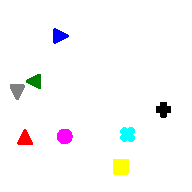
\includegraphics[width=0.235\textwidth]{figures/diversity/2.png}\\
  Output A& Output B\\
  \end{tabular}
  \caption{diversity.}
\label{fig:diversity}
\end{figure}


\section{Baselines}
\label{sec:baselines}
%\vspace{\sectionReduceTop}
\section{VQA Baselines and Methods}
%\vspace{\sectionReduceBot}
\begin{figure*}[h]
\includegraphics[width=1\linewidth]{figures/best_model_compressed.pdf}
\centering
\caption{Our best performing model (deeper LSTM Q + norm I). This model uses a two layer LSTM to encode the questions and the last hidden layer of VGGNet~\cite{Simonyan14c} to encode the images. The image features are then $\ell_2$ normalized. Both the question and image features are transformed to a common space and fused via element-wise multiplication, which is then passed through a fully connected layer followed by a softmax layer to obtain a distribution over answers.}
\label{fig:best_model}
%\vspace{\captionReduceBot}
\end{figure*}
In this section, we explore the difficulty of the VQA dataset for the MS COCO images using several baselines 
and novel methods. We train on VQA train+val. Unless stated otherwise, all human accuracies are on test-standard, machine accuracies are on test-dev, and results involving human captions (in gray font) are trained on train and tested on val (because captions are not available for test). 

\subsection{Baselines}
\label{sec:baselinesmain}
We implemented the following baselines:
\begin{enumerate}
\item \textbf{random:} We randomly choose an answer from the top 1K answers of the VQA train/val dataset.

\item \textbf{prior (``yes''):} We always select the most popular answer (``yes'') for both the open-ended and multiple-choice tasks. Note that ``yes'' is always one of the choices for the multiple-choice questions.

\item \textbf{per Q-type prior:} For the open-ended task, we pick the most popular answer per question type (see the appendix for details). For the multiple-choice task, we pick the answer (from the provided choices) that is most similar to the picked answer for the open-ended task using cosine similarity in Word2Vec\cite{word2vec} feature space.

\item \textbf{nearest neighbor:} Given a test image, question pair, we first find the $K$ nearest neighbor questions and associated images from the training set. See appendix for details on how neighbors are found. Next, for the open-ended task, we pick the most frequent ground truth answer from this set of nearest neighbor question, image pairs. Similar to the ``per Q-type prior'' baseline, for the multiple-choice task, we pick the answer (from the provided choices) that is most similar to the picked answer for the open-ended task using cosine similarity in \\ Word2Vec\cite{word2vec} feature space.
\end{enumerate}

%If we randomly choose an answer from the top 1K answers of the VQA train/val dataset, 
%the test-standard accuracy is $0.12\%$. 
%If we always select the most popular answer (``yes''), the accuracy is $29.72\%$. Picking the most popular answer per question type does $37.55\%$ and a nearest neighbor approach does $42.73\%$ on test-standard (see the appendix for details).
%For testing, we use the same train/val/test splits as COCO$^2$. 
%we split our real image dataset into a training and testing dataset. Our training dataset contains $30,000$ images and our testing dataset contains $20,000$ images. \jiasen{change image numbers, also including the NN baseline?}
\vspace{-5pt}
\subsection{Methods}
\label{sec:methods}
For our methods, we develop a 2-channel vision (image) + language (question) model that culminates with a softmax over $K$ possible outputs. We choose the top $K = 1000$ most frequent answers as possible outputs. This set of answers covers $82.67\%$ of the train+val answers. We describe the different components of our model below:

\textbf{Image Channel:} This channel provides an embedding for the image. We experiment with two embeddings -- 
\begin{compactenum}
\item \textbf{I:} The activations from the last hidden layer of VGGNet~\cite{Simonyan14c} are used as 4096-dim image embedding.
\item \textbf{norm I:} These are $\ell_2$ normalized activations from the last hidden layer of VGGNet~\cite{Simonyan14c}.
\end{compactenum}

\textbf{Question Channel:} This channel provides an embedding for the question. We experiment with three embeddings --
\begin{compactenum}
\item \textbf{Bag-of-Words Question (BoW Q)}: The top 1,000 words in the questions are used to create a bag-of-words representation. Since there is a strong correlation between the words that start a question and the answer (see \figref{fig:AnsPerQues}), we find the top 10 first, second, and third words of the questions and create a 30 dimensional bag-of-words representation. These features are concatenated to get a 1,030-dim embedding for the question.
\item \textbf{LSTM Q:} An LSTM with one hidden layer is used to obtain 1024-dim embedding for the question. The embedding obtained from the LSTM is a concatenation of last cell state and last hidden state representations (each being 512-dim) from the hidden layer of the LSTM. Each question word is encoded with 300-dim embedding by a fully-connected layer + tanh non-linearity which is then fed to the LSTM. The input vocabulary to the embedding layer consists of all the question words seen in the training dataset.
\item \textbf{deeper LSTM Q:} An LSTM with two hidden layers is used to obtain 2048-dim embedding for the question. The embedding obtained from the LSTM is a concatenation of last cell state and last hidden state representations (each being 512-dim) from each of the two hidden layers of the LSTM. Hence 2 (hidden layers) x 2 (cell state and hidden state) x 512 (dimensionality of each of the cell states, as well as hidden states) in \figref{fig:best_model}. This is followed by a fully-connected layer + tanh non-linearity to transform 2048-dim embedding to 1024-dim. The question words are encoded in the same way as in LSTM Q.   
\end{compactenum}

\textbf{Multi-Layer Perceptron (MLP):} The image and question embeddings 
%obtained from the image and question channels respectively 
are combined to obtain a single embedding. 
\begin{compactenum}
\item For \textbf{BoW Q + I} method, we simply concatenate the BoW Q and I embeddings. 
\item For \textbf{LSTM Q + I}, and \textbf{deeper LSTM Q + norm I} (\figref{fig:best_model}) methods, the image embedding is first transformed to 1024-dim by a fully-connected layer + tanh non-linearity to match the LSTM embedding of the question. The transformed image and LSTM embeddings (being in a common space) are then fused via element-wise multiplication. 
\end{compactenum}
This combined image + question embedding is then passed to an MLP -- a fully connected neural network classifier with 2 hidden layers and 1000 hidden units (dropout 0.5) in each layer with tanh non-linearity, followed by a softmax layer to obtain a distribution over $K$ answers. The entire model is learned end-to-end with a cross-entropy loss. VGGNet parameters are frozen to those learned for ImageNet classification and not fine-tuned in the image channel.   

We also experimented with providing captions as input to our model. Similar to \tableref{table:commonsense_acc}, we assume that a human-generated caption is given as input. We use a bag-of-words representation containing the 1,000 most popular words in the captions as the caption embedding (\textbf{Caption}). For \textbf{BoW Question + Caption (BoW Q + C)} method, we simply concatenate the BoW Q and C embeddings. 
%\jiasen{We don't know the coverage on test set, should we report the coverage on train+val set?} All baselines train a softmax neural network classifier with a single hidden layer containing 50 units. \jiasen{We have MLP baseline and LSTM baseline. For the MLP baseline, we train a softmax neural network classifier with 2 hidden layer each containing 1000 units. We use Tanh() as non-linear function and apply Dropout with probability 0.5 in each hidden layer.} 
%We experiment with three models: 
%(i) a multi-layer perceptron (MLP) neural network classifier with 2 hidden layers and 1000 hidden 
%units (dropout 0.5) in each layer with tanh non-linearity,  
%(ii) an LSTM model followed by a softmax layer to obtain a distribution over answers, and
%(iii) a two layer deeper LSTM model followed by softmax layer to obtain a distribution over answers.
%We experimented with five inputs for the MLP model. \textbf{Bag-of-Words Question (BoW Q)}: The top 1,000 words in the questions are used to create a bag-of-words representation. Since there is a strong correlation between the words that start a question and the answer (see \figref{fig:AnsPerQues}), we find the top 10 first, second, and third words of the questions and create a 30 dimensional bag-of-words representation. These features are concatenated to get a 1,030 dimensional input representation. \textbf{Caption:} Similar to \tableref{table:commonsense_acc}, we assume that a human-generated caption is given as input. We use a bag-of-words representation containing the 1,000 most popular words in the captions as the input feature. \textbf{Image (I):} We use the last hidden layer of VGGNet~\cite{Simonyan14c} as our 4096-dim feature. We also report the learned baseline results on \textbf{BoW Question + Image (BoW Q + I)} and \textbf{BoW Question + Caption (BoW Q + C)} by simply concatenating the first hidden layer representations of networks trained on each feature individually. The LSTM model uses a one-hot encoding for the question words, and the same image features as above followed by a linear + tanh transformation to transform the image features to 1024 dimensions to match the LSTM encoding of the question. The question and image encodings are fused via element-wise multiplication. The deeper LSTM Q model uses two hidden layers in the LSTM unlike only one hidden layer in the LSTM model. The deeper LSTM Q + norm I model (\figref{fig:best_model}) has almost the same architecture as the LSTM Q + I model except that it uses deeper LSTM (two hidden layer) and $l2$ normalized image features.

%For LSTM question only baseline, we simply input the question words into the LSTM along and fed into a softmax layer at the last timestep to generate the answers. For the LSTM vis baseline, we use the same VGG Conv Net fc7 layer feature, and use a linear trainsforamtion to map 4096 dimension image feature vectors to 1024 dimensional vector that match the dimension of encoded question feature. We fuse the image and question feature by doing an element-wise multiplication and further fed into a softmax layer. } 
For testing, we report the result on two different tasks: open-ended selects the answer with highest activation from all possible $K$ answers and multiple-choice picks the answer that has the highest activation from the potential answers. 

\subsection{Results}
\label{sec:results}

\begin{table}[t] \scriptsize
\setlength{\tabcolsep}{1.8pt}
\begin{center}
\begin{tabular}{@{} l  c  c  c  c  c  c c c@{}}
%\hline
\toprule
& \multicolumn{4}{c}{Open-Ended} & \multicolumn{4}{c}{ Multiple-Choice} \\

\cmidrule[0.75pt](l){2-5}
\cmidrule[0.75pt](l){6-9}
 & All & Yes/No & Number & Other & All & Yes/No & Number & Other \\
%\hline
\midrule
prior (``yes'') & 29.66 & 70.81 & 00.39 & 01.15 & 29.66 & 70.81 & 00.39 & 01.15 \\
per Q-type prior & 37.54 & 71.03 & 35.77 & 09.38 &  39.45 & 71.02 & 35.86 & 13.34 \\
nearest neighbor & 42.70 & 71.89 & 24.36 & 21.94 & 48.49 & 71.94 & 26.00 & 33.56 \\
BoW Q & \textcolor{black}{48.09} & \textcolor{black}{75.66} &  \textcolor{black}{36.70}& \textcolor{black}{27.14} 
& \textcolor{black}{53.68} & \textcolor{black}{75.71} & \textcolor{black}{37.05} & \textcolor{black}{38.64}\\
I & \textcolor{black}{28.13} & \textcolor{black}{64.01} & 00.42 & \textcolor{black}{03.77}  
&\textcolor{black}{30.53} & \textcolor{black}{69.87} & 00.45 & \textcolor{black}{03.76}\\
BoW Q + I & \textcolor{black}{52.64} & \textcolor{black}{75.55} & 33.67 & \textcolor{black}{37.37} 
& \textcolor{black}{58.97} & \textcolor{black}{75.59} & 34.35 & \textcolor{black}{50.33}\\
LSTM Q & \textcolor{black}{48.76} & \textcolor{black}{78.20} & 35.68 & \textcolor{black}{26.59} 
& \textcolor{black}{54.75} & \textcolor{black}{78.22} & 36.82 &\textcolor{black}{38.78}\\
LSTM Q + I & \textcolor{black}{53.74} & \textcolor{black}{78.94} & 35.24 & \textcolor{black}{36.42} 
& \textcolor{black}{57.17} & \textcolor{black}{78.95}& 35.80 & \textcolor{black}{43.41}\\
deeper LSTM Q & \textcolor{black}{50.39} & \textcolor{black}{78.41} & 34.68 & \textcolor{black}{30.03} 
& \textcolor{black}{55.88} & \textcolor{black}{78.45} & 35.91 &\textcolor{black}{41.13}\\
%\textcolor{red}{deeper LSTM Q} \\
deeper LSTM Q + norm I & \textbf{57.75} & \textbf{80.50} & \textbf{36.77} & \textbf{43.08} 
& \textbf{62.70} & \textbf{80.52}& \textbf{38.22} & \textbf{53.01}\\
%\textcolor{red}{norm I} \\
\midrule
\textcolor{gray}{Caption} & \textcolor{gray}{26.70} & \textcolor{gray}{65.50} & \textcolor{gray}{02.03} & \textcolor{gray}{03.86} 
& \textcolor{gray}{28.29} & \textcolor{gray}{69.79} & \textcolor{gray}{02.06} & \textcolor{gray}{03.82}\\
\textcolor{gray}{BoW Q + C} & \textcolor{gray}{54.70} & \textcolor{gray}{75.82} & \textcolor{gray}{40.12} & \textcolor{gray}{42.56} 
& \textcolor{gray}{59.85} & \textcolor{gray}{75.89} & \textcolor{gray}{41.16}  & \textcolor{gray}{52.53}\\
\bottomrule
\end{tabular}	
\caption{Accuracy of our methods for the open-ended and multiple-choice tasks on the VQA test-dev for real images. 
Q = Question, I = Image, C = Caption. (Caption and BoW Q + C results are on val). 
See text for details.
}
%\vspace{-10pt}
\label{tab:acc}
\end{center}
\end{table}
\tableref{tab:acc} shows the accuracy of our baselines and methods for both the open-ended and multiple-choice tasks on the VQA test-dev for real images.

As expected, the vision-alone model (I) that completely ignores the question performs rather poorly (open-ended: 28.13\% / multiple-choice: 30.53\%). In fact, on open-ended task, the vision-alone model (I) performs worse than the prior (``yes'') baseline, which ignores both the image \emph{and} question (responding to every question with a ``yes''). 

Interestingly, the language-alone methods (per Q-type prior, BoW Q, LSTM Q) that ignore the image perform surprisingly well, with BoW Q achieving 48.09\% on open-ended (53.68\% on multiple-choice) and LSTM Q achieving 48.76\% on open-ended (54.75\% on multiple-choice); both outperforming the nearest neighbor baseline (open-ended: 42.70\%, multiple-choice: 48.49\%). Our quantitative results and analyses suggest that this might be due to the language-model exploiting subtle statistical priors about the question types (e.g. ``What color is the banana?'' can be answered with ``yellow'' without looking at the image). For a detailed discussion of the subtle biases in the questions, please see \cite{yinyang}. 

The accuracy of our \textbf{best model} (deeper LSTM Q + norm I (\figref{fig:best_model}), selected using VQA test-dev accuracies) on VQA test-standard is 58.16\% (open-ended) / 63.09\% (multiple-choice). We can see that our model is able to significantly outperform both the vision-alone and language-alone baselines. As a general trend, results on multiple-choice are better than open-ended. All methods are significantly worse than human performance.
%The accuracy of our \textbf{best model} (deeper LSTM Q + norm I (\figref{fig:best_model}), selected using VQA test-dev accuracies) on VQA test-standard is $\textbf{58.16\%}$.
%The accuracy using only the question is $\sim$48\%, which demonstrates that the type of question is informative of the answer. As expected, results on multiple-choice are better than open-ended. 
%%In comparison to 
%All methods are significantly worse than human performance. 

Our VQA demo is available on CloudCV \cite{cloudcv} -- \url{http://cloudcv.org/vqa}. This will be updated with newer models as we develop them.

%\textcolor{red}{In \tableref{tab:acc}, the results of (Q + I) are very similar to the results of only using the questions, while the addition of captions (Q + C) provides minimal improvement $\sim2-4\%$.} 
To gain further insights into these results, we computed accuracies by question type in \tableref{tab:typeacc}. Interestingly, for question types that require more reasoning, such as ``Is the'' or ``How many'', the scene-level image features do not provide any additional information. However, for questions that can be answered using scene-level information, such as ``What sport,'' 
%or ``What animal''
we do see an improvement. Similarly, for questions whose answer may be contained in a generic caption we see improvement, such as ``What animal''. For all question types, the results are worse than human accuracies.

We also analyzed the accuracies of our best model (deeper LSTM Q + norm I) on a subset of questions with certain specific (ground truth) answers. In \figref{fig:prob_1}, we show the average accuracy of the model on questions with 50 most frequent ground truth answers on the VQA validation set (plot is sorted by accuracy, not frequency). We can see that the model performs well for answers that are common visual objects such as ``wii'', ``tennis'', ``bathroom'' while the performance is somewhat underwhelming for counts (\eg, ``2'', ``1'', ``3''), and particularly poor for higher counts (\eg, ``5'', ``6'', ``10'', ``8'', ``7''). 

In \figref{fig:prob_2}, we show the distribution of 50 most frequently predicted answers when the system is correct on the VQA validation set (plot is sorted by prediction frequency, not accuracy). In this analysis, ``system is correct'' implies that it has VQA accuracy $1.0$ (see section \ref{sec:dataset} for accuracy metric). We can see that the frequent ground truth answers (\eg, ``yes'', ``no'', ``2'', ``white'', ``red'', ``blue'', ``1'', ``green'') are more frequently predicted than others when the model is correct. 

%This observation suggests that the model is probably learning the distribution of answers in the training dataset.

%%%%%%%%%%%%%%%%%%%%%%%%%%%%%%%%%%%%%%%%%%%%%%%%%%%%%%%%%


\begin{table}[h] \scriptsize
\setlength{\tabcolsep}{2pt}
\begin{center}
\begin{tabular}{@{} l  c  c  c  c c c c@{}  }
%\hline
\toprule
& \multicolumn{5}{c}{Open-Ended}   & Human Age & Commonsense\\

%\cline{2-6}
\cmidrule[0.9pt](l){2-6}

\multicolumn{1}{c}{Question} & \multicolumn{3}{c}{K = 1000} & \multicolumn{2}{c}{Human} & To Be Able & To Be Able\\
\cmidrule[0.5pt](lr){2-4}
\cmidrule[0.5pt](l){5-6}

\multicolumn{1}{c}{Type}  & Q & Q + I & Q + C & Q & Q + I & To Answer & To Answer (\%)\\
%\hline
\midrule
what is \textcolor{black}{(13.84)} & \textcolor{black}{23.57} & \textcolor{black}{34.28} & \textcolor{gray}{43.88} & \textcolor{black}{16.86} & \textcolor{black}{73.68} &\textcolor{black}{09.07} & 27.52\\
what color \textcolor{black}{(08.98)} & \textcolor{black}{33.37} & \textcolor{black}{43.53} & \textcolor{gray}{48.61} & \textcolor{black}{28.71} & \textcolor{black}{86.06} &\textcolor{black}{06.60} & 13.22\\
what kind \textcolor{black}{(02.49)} & \textcolor{black}{27.78} & \textcolor{black}{42.72} & \textcolor{gray}{43.88} & \textcolor{black}{19.10} & \textcolor{black}{70.11} &\textcolor{black}{10.55} & 40.34\\
what are \textcolor{black}{(02.32)} & \textcolor{black}{25.47} & \textcolor{black}{39.10} & \textcolor{gray}{47.27} & \textcolor{black}{17.72} & \textcolor{black}{69.49} &\textcolor{black}{09.03} & 28.72\\
what type \textcolor{black}{(01.78)} & \textcolor{black}{27.68} & \textcolor{black}{42.62} & \textcolor{gray}{44.32} & \textcolor{black}{19.53} & \textcolor{black}{70.65} &\textcolor{black}{11.04} & 38.92\\
is the \textcolor{black}{(10.16)} & \textcolor{black}{70.76} & \textcolor{black}{69.87} & \textcolor{gray}{70.50} & \textcolor{black}{65.24} & \textcolor{black}{95.67} &\textcolor{black}{08.51} & 30.30\\
is this \textcolor{black}{(08.26)} & \textcolor{black}{70.34} & \textcolor{black}{70.79} & \textcolor{gray}{71.54} & \textcolor{black}{63.35} & \textcolor{black}{95.43} &\textcolor{black}{10.13} & 45.32\\
how many \textcolor{black}{(10.28)} & \textcolor{black}{43.78} & \textcolor{black}{40.33} & \textcolor{gray}{47.52} & \textcolor{black}{30.45} & \textcolor{black}{86.32} &\textcolor{black}{07.67}& 15.93 \\
are \textcolor{black}{(07.57)} & \textcolor{black}{73.96} & \textcolor{black}{73.58} & \textcolor{gray}{72.43} & \textcolor{black}{67.10} & \textcolor{black}{95.24} &\textcolor{black}{08.65} & 30.63\\
does \textcolor{black}{(02.75)} & \textcolor{black}{76.81} & \textcolor{black}{75.81} & \textcolor{gray}{75.88} & \textcolor{black}{69.96} & \textcolor{black}{95.70} &\textcolor{black}{09.29} & 38.97\\
where \textcolor{black}{(02.90)} & \textcolor{black}{16.21} & \textcolor{black}{23.49} & \textcolor{gray}{29.47} & \textcolor{black}{11.09} & \textcolor{black}{43.56} &\textcolor{black}{09.54} & 36.51\\
is there \textcolor{black}{(03.60)} & \textcolor{black}{86.50} & \textcolor{black}{86.37} & \textcolor{gray}{85.88} & \textcolor{black}{72.48} & \textcolor{black}{96.43} &\textcolor{black}{08.25} & 19.88\\
why \textcolor{black}{(01.20)} & \textcolor{black}{16.24} & \textcolor{black}{13.94} & \textcolor{gray}{14.54} & \textcolor{black}{11.80} & \textcolor{black}{21.50} &\textcolor{black}{11.18} & 73.56\\
which \textcolor{black}{(01.21)} & \textcolor{black}{29.50} & \textcolor{black}{34.83} & \textcolor{gray}{40.84} & \textcolor{black}{25.64} & \textcolor{black}{67.44} &\textcolor{black}{09.27} & 30.00\\
do \textcolor{black}{(01.15)} & \textcolor{black}{77.73} & \textcolor{black}{79.31} & \textcolor{gray}{74.63} & \textcolor{black}{71.33} & \textcolor{black}{95.44} &\textcolor{black}{09.23} & 37.68\\
what does \textcolor{black}{(01.12)} & \textcolor{black}{19.58} & \textcolor{black}{20.00} & \textcolor{gray}{23.19} & \textcolor{black}{11.12} & \textcolor{black}{75.88} &\textcolor{black}{10.02} & 33.27\\
what time \textcolor{black}{(00.67)} & \textcolor{black}{8.35} & \textcolor{black}{14.00} & \textcolor{gray}{18.28} & \textcolor{black}{07.64} & \textcolor{black}{58.98} &\textcolor{black}{09.81} & 31.83\\
who \textcolor{black}{(00.77)} & \textcolor{black}{19.75} & \textcolor{black}{20.43} & \textcolor{gray}{27.28} & \textcolor{black}{14.69} & \textcolor{black}{56.93} &\textcolor{black}{09.49} & 43.82\\
what sport \textcolor{black}{(00.81)} & \textcolor{black}{37.96} & \textcolor{black}{81.12} & \textcolor{gray}{93.87} & \textcolor{black}{17.86} & \textcolor{black}{95.59} &\textcolor{black}{08.07} & 31.87\\
what animal \textcolor{black}{(00.53)} & \textcolor{black}{23.12} & \textcolor{black}{59.70} & \textcolor{gray}{71.02} & \textcolor{black}{17.67} & \textcolor{black}{92.51} &\textcolor{black}{06.75} & 18.04\\
what brand \textcolor{black}{(00.36)} & \textcolor{black}{40.13} & \textcolor{black}{36.84} & \textcolor{gray}{32.19} & \textcolor{black}{25.34} & \textcolor{black}{80.95} &\textcolor{black}{12.50} & 41.33\\
                                                                                                                                                             
\bottomrule
\end{tabular}
\caption{Open-ended test-dev results for different question types on real images (Q+C is reported on val).
Machine performance is reported using the bag-of-words representation for questions.
Questions types are determined by the one or two words that start the question. 
The percentage of questions for each type is shown in parentheses. 
%All results are the percentage of answers in agreement with human subjects. 
Last and second last columns respectively show the average human age and average degree of commonsense required to answer the questions 
(as reported by AMT workers), respectively. 
See text for details.}
\vspace{-10pt}
\label{tab:typeacc}
\end{center}
\end{table}
%%%%%%%%%%%%%%%%%%%%%%%%%%%%%%%%%%%%%%%%%%%%%%%%%%%%%%%%%

%We also tested our baselines on only binary $K=2$ (\ie, ``yes/no'' questions). The results are shown in \tableref{tab:acc} (right column). The results generally improve upon the baseline of answering ``yes'' to every question (\textcolor{red}{$66.97\%$}). However, they are again significantly worse than human performance.

Finally, evaluating our best model (deeper LSTM Q + norm I) on the validation questions for which we have age annotations (how old a human needs to be to answer the question correctly), we estimate that our model performs as well as a $4.74$ year old child! The average age required on the same set of questions is $8.98$. Evaluating the same model on the validation questions for which we have commonsense annotations (whether the question requires commonsense to answer it), we estimate that it has degree of commonsense of $17.35\%$. The average degree of commonsense required on same set of questions is $31.23\%$. Again, these estimates reflect the age and commonsense perceived by MTurk workers that would be required to answer the question. See the appendix for details. 

We further analyzed the performance of the model for different age groups on the validation questions for which we have age annotations. In \figref{fig:age_1}, we computed the average accuracy of the predictions made by the model for questions belonging to different age groups. Perhaps as expected, the accuracy of the model decreases as the age of the question increases (from $61.07\%$ at $3-4$ age group to $47.83\%$ at $18+$ age group). 

In \figref{fig:age_2}, we show the distribution of age of questions for different levels of accuracies achieved by our system on the validation questions for which we have age annotations. It is interesting to see that the relative proportions of different age groups is consistent across all accuracy bins with questions belonging to the age group 5-8 comprising the majority of the predictions which is expected because 5-8 is the most common age group in the dataset (see \figref{fig:age}).

%\begin{figure*}[t]
%\includegraphics[width=1\linewidth]{figures/prob1_sorted_pvalues_OpenEnded_val2014.pdf}
%\centering
%\caption{$\Pr\text{(system is correct }|\text{ answer\_i)}$ for 50 most accurate answers.}
%\label{fig:prob_1_sorted_pvalues}
%%\vspace{\captionReduceBot}
%\end{figure*}
\begin{figure*}[h]
\includegraphics[width=1\linewidth]{figures/prob1_OpenEnded_val2014_sorted.pdf}
\centering
\caption{$\Pr\text{(system is correct } | \text{ answer)}$ for 50 most frequent ground truth answers on the VQA validation set (plot is sorted by accuracy, not frequency). System refers to our best model (deeper LSTM Q + norm I).}
\label{fig:prob_1}
%\vspace{\captionReduceBot}
\end{figure*}
\begin{figure*}[h]
\includegraphics[width=1\linewidth]{figures/prob2_OpenEnded_val2014_100_logscale.pdf}
\centering
\caption{$\Pr\text{(answer } | \text{ system is correct)}$ for 50 most frequently predicted answers on the VQA validation set (plot is sorted by prediction frequency, not accuracy). System refers to our best model (deeper LSTM Q + norm I).}
\label{fig:prob_2}
%\vspace{\captionReduceBot}
\end{figure*}
\begin{figure}[h]
\includegraphics[width=1\linewidth]{figures/OpenEnded_val2014_predAgeDict2.pdf}
\centering
\caption{$\Pr\text{(system is correct } | \text{ age of question)}$ on the VQA validation set. System refers to our best model (deeper LSTM Q + norm I).}
\label{fig:age_1}
%\vspace{\captionReduceBot}
\end{figure}
\begin{figure}[h]
\includegraphics[width=1\linewidth]{figures/OpenEnded_val2014_predAgeDict1.pdf}
\centering
\caption{$\Pr\text{(age of question } | \text{ system is correct)}$ on the VQA validation set. System refers to our best model (deeper LSTM Q + norm I).}
\label{fig:age_2}
%\vspace{\captionReduceBot}
\end{figure}

\tableref{tab:abl_acc} shows the accuracy of different ablated versions of our best model (deeper LSTM Q + norm I) for both the open-ended and multiple-choice tasks on the VQA test-dev for real images. The different ablated versions are as follows --

\begin{compactenum}
\item \textbf{Without I Norm:} In this model, the activations from the last hidden layer of VGGNet~\cite{Simonyan14c} are not $\ell_2$-normalized. Comparing the accuracies in \tableref{tab:abl_acc} and \tableref{tab:acc}, we can see that $\ell_2$-normalization of image features boosts the performance by 0.16\% for open-ended task and by 0.24\% for multiple-choice task. 

\item \textbf{Concatenation:} In this model, the transformed image and LSTM embeddings are concatenated (instead of element-wise multiplied), resulting in doubling the number of parameters in the following fully-connected layer. Comparing the accuracies in \tableref{tab:abl_acc} and \tableref{tab:acc}, we can see that element-wise fusion performs better by 0.95\% for open-ended task and by 1.24\% for multiple-choice task.

\item \textbf{K = 500:} In this model, we use K = 500 most frequent answers as possible outputs. Comparing the accuracies in \tableref{tab:abl_acc} and \tableref{tab:acc}, we can see that K = 1000 performs better than K = 500 by 0.82\% for open-ended task and by 1.92\% for multiple-choice task.

\item \textbf{K = 2000:} In this model, we use K = 2000 most frequent answers as possible outputs. Comparing the accuracies in \tableref{tab:abl_acc} and \tableref{tab:acc}, we can see that K = 2000 performs better then K = 1000 by 0.40\% for open-ended task and by 1.16\% for multiple-choice task.

\item \textbf{Truncated Q Vocab $@$ 5:} In this model, the input vocabulary to the embedding layer (which encodes the question words) consists of only those question words which occur atleast 5 times in the training dataset, thus reducing the vocabulary size from 14770 (when all question words are used) to 5134 (65.24\% reduction). Remaining question words are replaced with UNK (unknown) tokens. Comparing the accuracies in \tableref{tab:abl_acc} and \tableref{tab:acc}, we can see that truncating the question vocabulary $@$ 5 performs better than using all questions words by 0.24\% for open-ended task and by 0.17\% for multiple-choice task.

\item \textbf{Truncated Q Vocab $@$ 11:} In this model, the input vocabulary to the embedding layer (which encodes the question words) consists of only those question words which occur atleast 11 times in the training dataset, thus reducing the vocabulary size from 14770 (when all question words are used) to 3561 (75.89\% reduction). Remaining question words are replaced with UNK (unknown) tokens. Comparing the accuracies in \tableref{tab:abl_acc} and \tableref{tab:acc}, we can see that truncating the question vocabulary $@$ 11 performs better than using all questions words by 0.06\% for open-ended task and by 0.02\% for multiple-choice task.

\item \textbf{Filtered Dataset:} We created a filtered version of the VQA train + val dataset in which we only keep the answers with subject confidence ``yes''. Also, we keep only those questions for which at least 50\% (5 out of 10) answers are annotated with subject confidence ``yes''. The resulting filtered dataset consists of 344600 questions, compared to 369861 questions in the original dataset, thus leading to only 6.83\% reduction in the size of the dataset. The filtered dataset has 8.77 answers per question on average. We did not filter the test set so that accuracies of the model trained on the filtered dataset can be compared with that of the model trained on the original dataset. The row ``Filtered Dataset'' in \tableref{tab:abl_acc} shows the performance of the deeper LSTM Q + norm I model when trained on the filtered dataset. Comparing these accuracies with the corresponding accuracies in \tableref{tab:acc}, we can see that the model trained on filtered version performs worse by 1.13\% for open-ended task and by 1.88\% for multiple-choice task.
\end{compactenum}

\begin{table}[t] \scriptsize
\setlength{\tabcolsep}{1.8pt}
\begin{center}
\begin{tabular}{@{} l  c  c  c  c  c  c c c@{}}
%\hline
\toprule
& \multicolumn{4}{c}{Open-Ended} & \multicolumn{4}{c}{Multiple-Choice} \\

\cmidrule[0.75pt](l){2-5}
\cmidrule[0.75pt](l){6-9}
 & All & Yes/No & Number & Other & All & Yes/No & Number & Other \\
%\hline
\midrule
Without I Norm & 57.59 & 80.41 & 36.63 & 42.84 & 62.46 & 80.43 & 38.10 & 52.62 \\
Concatenation & 56.80 & 78.49 & 35.08 & 43.19 & 61.46 & 78.52 & 36.43 & 52.54 \\
K = 500 & 56.93 & 80.61 & 36.24 & 41.39 & 60.78 & 80.64 & 37.44 & 49.10 \\
K = 2000 & 58.15 & 80.56 & 37.04 & 43.79 & 63.86 & 80.59 & 38.97 & 55.20 \\
Truncated Q Vocab $@$ 5 & 57.99 & 80.67 & 36.99 & 43.38 & 62.87 & 80.71 & 38.22 & 53.20\\
Truncated Q Vocab $@$ 11 & 57.81 & 80.42 & 36.97 & 43.22 & 62.72 & 80.45 & 38.30 & 53.09\\
Filtered Dataset & 56.62 & 80.19 & 37.48 & 40.95 & 60.82 & 80.19 & 37.48 & 49.57 \\
\bottomrule
\end{tabular}	
\caption{Accuracy of ablated versions of our best model (deeper LSTM Q + norm I) for the open-ended and multiple-choice tasks on the VQA test-dev for real images. 
Q = Question, I = Image. 
See text for details.
}
%\vspace{-10pt}
\label{tab:abl_acc}
\end{center}
\end{table}

\section{Experiments}
\label{sec:experiments}
% !TEX root = ../multi_task.tex

We evaluate the presented MTL method on a number of problems. First, we use MultiMNIST \citep{multi_mnist}, an MTL adaptation of MNIST \citep{mnist}. Next, we tackle multi-label classification on the CelebA dataset \citep{celeba} by considering each label as a distinct binary classification task. These problems include both classification and regression, with the number of tasks ranging from 2 to 40. Finally, we experiment with scene understanding, jointly tackling the tasks of semantic segmentation, instance segmentation, and depth estimation on the Cityscapes dataset \citep{cityscapes}. We discuss each experiment separately in the following subsections.

The baselines we consider are (i) \textbf{uniform scaling:} minimizing a uniformly weighted sum of loss functions \mbox{$\frac{1}{T}\sum_t \lL^t$}, \mbox{(ii) \textbf{single task:}} solving tasks independently, \mbox{(iii) \textbf{grid search:}} exhaustively trying various values from $\{ c^t \in [0,1] | \sum_t c^t = 1\}$ and optimizing for $\frac{1}{T}\sum_t c^t \lL^t$, \mbox{(iv) \textbf{\citet{Kendall2018}:}} using the uncertainty weighting proposed by \citet{Kendall2018}, and \mbox{(v) \textbf{GradNorm:}} using the normalization proposed by \citet{Chen2018}.



\subsection{MultiMNIST}
\label{sec:multi_mnist_exp}

Our initial experiments are on MultiMNIST, an MTL version of the MNIST dataset \citep{multi_mnist}. In order to convert digit classification into a multi-task problem, \citet{multi_mnist} overlaid multiple images together. We use a similar construction. For each image, a different one is chosen uniformly in random. Then one of these images is put at the top-left and the other one is at the bottom-right. The resulting tasks are: classifying the digit on the top-left (task-L) and classifying the digit on the bottom-right (task-R). We use 60K examples and directly apply existing single-task MNIST models. The MultiMNIST dataset is illustrated in the supplement.

We use the LeNet architecture \citep{mnist}. We treat all layers except the last as the representation function $g$ and put two fully-connected layers as task-specific functions (see the supplement for details). We visualize the performance profile as a scatter plot of accuracies on task-L and task-R in Figure~\ref{fig:multi_mnist_performance_curve}, and list the results in Table~\ref{tab:multi_mnist}.

In this setup, any static scaling results in lower accuracy than solving each task separately (the single-task baseline). The two tasks appear to compete for model capacity, since increase in the accuracy of one task results in decrease in the accuracy of the other. Uncertainty weighting \citep{Kendall2018} and GradNorm \citep{Chen2018} find solutions that are slightly better than grid search but distinctly worse than the single-task baseline. In contrast, our method finds a solution that efficiently utilizes the model capacity and yields accuracies that are as good as the single-task solutions. This experiment demonstrates the effectiveness of our method as well as the necessity of treating MTL as multi-objective optimization. Even after a large hyper-parameter search, \emph{any} scaling of tasks does not approach the effectiveness of our method.



\subsection{Multi-Label Classification}

\begin{figure}[t]
\includegraphics[width=\textwidth]{radar_full_new}
\vspace{1mm}
\caption{Radar charts of percentage error per attribute on CelebA \citep{celeba}. Lower is better. We divide attributes into two sets for legibility: easy on the left, hard on the right. Zoom in for details.}
\label{fig:multi_label_radar}
\end{figure}


\begin{wraptable}{r}{0.3\textwidth}
%\vspace{-4mm}
\captionof{table}{Mean of error per category of MTL algorithms in multi-label classification on CelebA \citep{celeba}.}
\begin{tabular}{r@{\hspace{2mm}}c@{}}
\toprule
& Average  \\
&  error \\
\midrule
Single task & $8.77$ \\
Uniform scaling & $9.62$ \\
\citealt{Kendall2018} & $9.53$ \\
GradNorm & $8.44$ \\
Ours & $\mathbf{8.25}$  \\
\bottomrule
\end{tabular}
\label{table:multi_label_bar}
%\vspace{-5mm}
\end{wraptable}

Next, we tackle multi-label classification. Given a set of attributes, multi-label classification calls for deciding whether each attribute holds for the input. We use the CelebA dataset \citep{celeba}, which includes 200K face images annotated with 40 attributes. Each attribute gives rise to a binary classification task and we cast this as a 40-way MTL problem. We use ResNet-18 \citep{resnet} without the final layer as a shared representation function, and attach a linear layer for each attribute (see the supplement for further details).


We plot the resulting error for each binary classification task as a radar chart in Figure~\ref{fig:multi_label_radar}. The average over them is listed in Table~\ref{table:multi_label_bar}. We skip grid search since it is not feasible over 40 tasks. Although uniform scaling is the norm in the multi-label classification literature, single-task performance is significantly better. Our method outperforms baselines for significant majority of tasks and achieves comparable performance in rest. This experiment also shows that our method remains effective when the number of tasks is high.


\subsection{Scene Understanding}

To evaluate our method in a more realistic setting, we use scene understanding. Given an RGB image, we solve three tasks: semantic segmentation (assigning pixel-level class labels), instance segmentation (assigning pixel-level instance labels), and monocular depth estimation (estimating continuous disparity per pixel). We follow the experimental procedure of \citet{Kendall2018} and use an encoder-decoder architecture. The encoder is based on ResNet-50 \citep{resnet} and is shared by all three tasks. The decoders are task-specific and are based on the pyramid pooling module \citep{pspnet} (see the supplement for further implementation details).

Since the output space of instance segmentation is unconstrained (the number of instances is not known in advance), we use a proxy problem as in \citet{Kendall2018}. For each pixel, we estimate the location of the center of mass of the instance that encompasses the pixel. These center votes can then be clustered to extract the instances. In our experiments, we directly report the MSE in the proxy task. Figure~\ref{fig:cityscapes_performance_profile} shows the performance profile for each pair of tasks, although we perform all experiments on all three tasks jointly. The pairwise performance profiles shown in Figure~\ref{fig:cityscapes_performance_profile} are simply 2D projections of the three-dimensional profile, presented this way for legibility. The results are also listed in Table~\ref{tab:cityscapes_results}.

MTL outperforms single-task accuracy, indicating that the tasks cooperate and help each other. Our method outperforms all baselines on all tasks.


\subsection{Role of the Approximation}

In order to understand the role of the approximation proposed in Section~\ref{sec:approximation}, we compare the final performance and training time of our algorithm with and without the presented approximation in Table~\ref{tab:approximation_tradeoff} (runtime measured on a single Titan Xp GPU). For a small number of tasks (3 for scene understanding), training time is reduced by 40\%. For the multi-label classification experiment (40 tasks), the presented approximation accelerates learning by a factor of 25.

On the accuracy side, we expect both methods to perform similarly as long as the full-rank assumption is satisfied. As expected, the accuracy of both methods is very similar. Somewhat surprisingly, our approximation results in slightly improved accuracy in all experiments. While counter-intuitive at first, we hypothesize that this is related to the use of SGD in the learning algorithm. Stability analysis in convex optimization suggests that if gradients are computed with an error $\hat{\nabla}_\btheta \mathcal{L}^t = \nabla_\btheta \mathcal{L}^t + \mathbf{e}^t$ ($\btheta$ corresponds to $\btheta^{sh}$ in (\ref{eq:kkt_opt})), as opposed to $\mathbf{Z}$ in the approximate problem in \ref{eq:approx}, the error in the solution is bounded as $\|\hat{\mathbf{\alpha}} - \mathbf{\alpha} \|_2 \leq \mathcal{O}(\max_t \|\mathbf{e}^t\|_2)$. Considering the fact that the gradients are computed over the full parameter set (millions of dimensions) for the original problem and over a smaller space for the approximation (batch size times representation which is in the thousands), the dimension of the error vector is significantly higher in the original problem. We expect the $l_2$ norm of such a random vector to depend on the dimension.

In summary, our quantitative analysis of the approximation suggests that (i) the approximation does not cause an accuracy drop and (ii) by solving an equivalent problem in a lower-dimensional space, our method achieves both better computational efficiency and higher stability.

  {\small
  \begin{table}[t]
%  \vspace{-4mm}
  \caption{Effect of the MGDA-UB approximation. We report the final accuracies as well as training times for our method with and without the approximation.}
  %\vspace{1mm}
  \centering
  \begin{tabular}{@{}r@{\hspace{3mm}}c@{\hspace{3mm}}c@{\hspace{2mm}}c@{\hspace{2mm}}c@{}c@{\hspace{5mm}}c@{\hspace{2mm}}c@{}}
  \toprule
  & \multicolumn{4}{c}{Scene understanding (3 tasks)} &  & \multicolumn{2}{c}{Multi-label (40 tasks)}  \\
  \cmidrule(r){2-5} \cmidrule(lr){7-8}
                  & Training & Segmentation & Instance  & Disparity      & & Training & Average \\
                 & time     &  mIoU [\%]       & error [px] & error [px] & & time (hour)      & error \\
  \midrule
  Ours (w/o approx.) & $38.6$ & $66.13$ & $10.28$ & $2.59$ & & $429.9$ & $8.33$ \\
  Ours & $\mathbf{23.3}$ & $\mathbf{66.63}$ & $\mathbf{10.25}$ & $\mathbf{2.54}$  & & $\mathbf{16.1}$ & $\mathbf{8.25}$ \\
  \bottomrule
  \end{tabular}
  %\vspace{-2mm}
  \label{tab:approximation_tradeoff}
  \end{table}}


\section{Conclusion}
\label{sec:discussion}
Though presented as an application paper, we have touched two fundamental problems: First, how to generate an orderless set of entities. Towards building generative models for more sophisticated combinatorial data structures such as graphs, knowing how to generate a set may be a good starting point. Second, how to capture the ambiguity of the groundtruth in a regression problem . Other than 3D reconstruction, many regression problems may have such inherent ambiguity. Our construction of the MoN loss by wrapping existing loss functions may be generalizable to these problems.


\balance

{\small
\bibliographystyle{ieee}
\bibliography{paper}
}

\end{document}
